\section{Method}
%----------------------- Method ----------------------------
\label{sec:method}

This section describes the steps and decisions taken towards the development of Sesnando. The concepts presented here are the result of the study of the state of the art and internal discussions with Project Advisors.


\subsection{Resource Analysis}
%----------------------- Resource Analysis ----------------------------
\label{subsec:resource_analysis}

This section presents the analysis procedures towards the available resources, namely, requirements sets. The Railway project used for this study stores its requirements on a Requirement Management Tool. Those requirements have been exported and analysed to extract relevant knowledge from them towards building a solid grammar that could satisfy these requirements logic.\\

It was not feasible to analyse such requirements one-by-one due to their number, so a tool has been developed to extract the needed data. First, the requirements have been exported in chunks of Excel files, but later, this same tool was able to directly access the requirement repository.

The requirement analysis tool has been developed using the following libraries.

\begin{itemize}
    \item pandas - For importing requirement files, data storage and data analysis.
    \item nltk - Natural Language Toolkit for data analysis.
    \item matplot - Data visualisation.
    \item xlswriter - To persist processed data.
\end{itemize}

The principal analysis taken was in the fields on the contiguous sequence and main requirement structures, for this, several models on N-Grams and Skip-grams have been generated.\\
N-gram model analysis are widely used in computational linguistics and communication theory such as Natural Language Processing (NLP) \cite{broder_syntactic_1997}.\\

The techniques to export the best N-gram models relied on arbitrary values and \textit{trial and error}. N-gram models above the value of 10 started to produce several repeating sequences, so the model analysis sat between the values of 2 and 10. Next is one of the N-gram Model where N = 10.

% width=\textwidth
\begin{figure}[H]
    \centering
    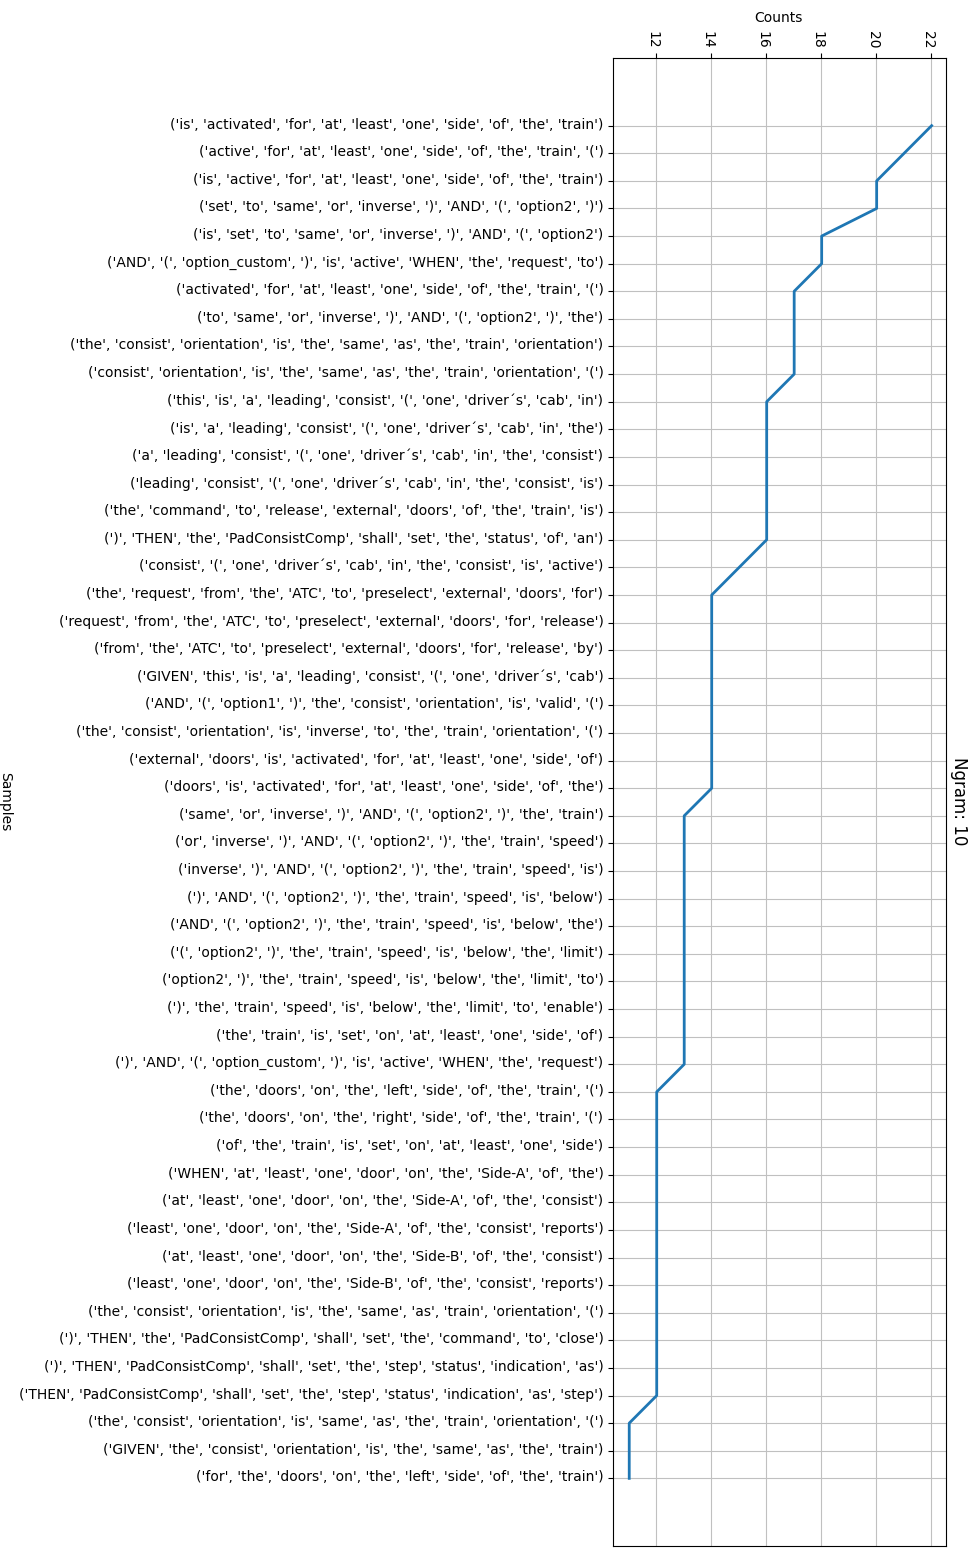
\includegraphics[scale=0.6]{images/n_gram10_cut.png}
    \caption{N-gram Model, N = 10}
    \label{fig:n_gram_model_10}
\end{figure}

The results of this analysis expressed the need of using logical boolean operators such as "AND" and "OR". Signal attributes such as "is active". Quantifiers containing their component/attribute and scope, as in "for at least one side of the train" and the \textit{THEN} condition in the form of "THEN the <Outcome Requirement signal> is set to \textit{VALUE}".
These have been used to define the requirements grammar, as presented on Section \ref{subsec:grammar_elements} (Grammar Elements) and Section \ref{sec:def_req_grammar} (Defining requirement grammar). In other words, the existing requirement structure and common natural instructions have been analysed to support the writing of a grammar that supports the same logic that is already presented on the existing requirements.

% width=\textwidth
\begin{figure}[H]
    \centering
    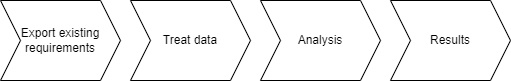
\includegraphics[width=\textwidth]{images/diag_ngram.png}
    \caption{Steps requirement analysis}
    \label{fig:diag_ngram_req_analysis}
\end{figure}

This analysis and obtained results involved the writing of an python program that took several sets of requirements as an input. The main activities are presented as bullet points.

\begin{itemize}
    \item Export existing requirements written in a natural language from the manufacturer requirement repository (IBM Doors).
    \item Treat existing requirements by anonymising Requirement Signals, so that, these do not influence the extraction of the most common used expressions.
    \item N-gram, Skip-gram and Stop-word analysis \cite{alajmi2012toward}.
    \item Analysis of the obtained results that enumerate a set of instructions that cover and support the most of the requirement logic already presented in a natural form.
\end{itemize}




\subsection{Defining the requirements grammar}
%----------------------- Defining the requirements grammar ----------------------------
\label{sec:def_req_grammar}

As the grammar lexer set has been identified it was then necessary to define an Abstract Syntax tree. It is known that \textit{GIVEN}, \textit{WHEN} and \textit{THEN} are the main predicates that define the skeleton of a requirement, thus, each predicate should implement its own Condition tree.\\
There are widely known libraries to support the building of a grammar, such as Flex and Bison \cite{levine_flex_2009}, however, flex and bison only work with C++ programs and Antlr works with a number of different languages \cite{antlr_site}, hence the choice of \textit{Antlr} library to support the development of this grammar. \textit{GIVEN}, \textit{WHEN} and \textit{THEN} are represented in the form of a Logical Expression that can be derived into child classes, given the lexer type. The representation of the syntax tree is presented on Figure \ref{fig:ast_class_diagram}.

% 
\begin{figure}[H]
    \centering
    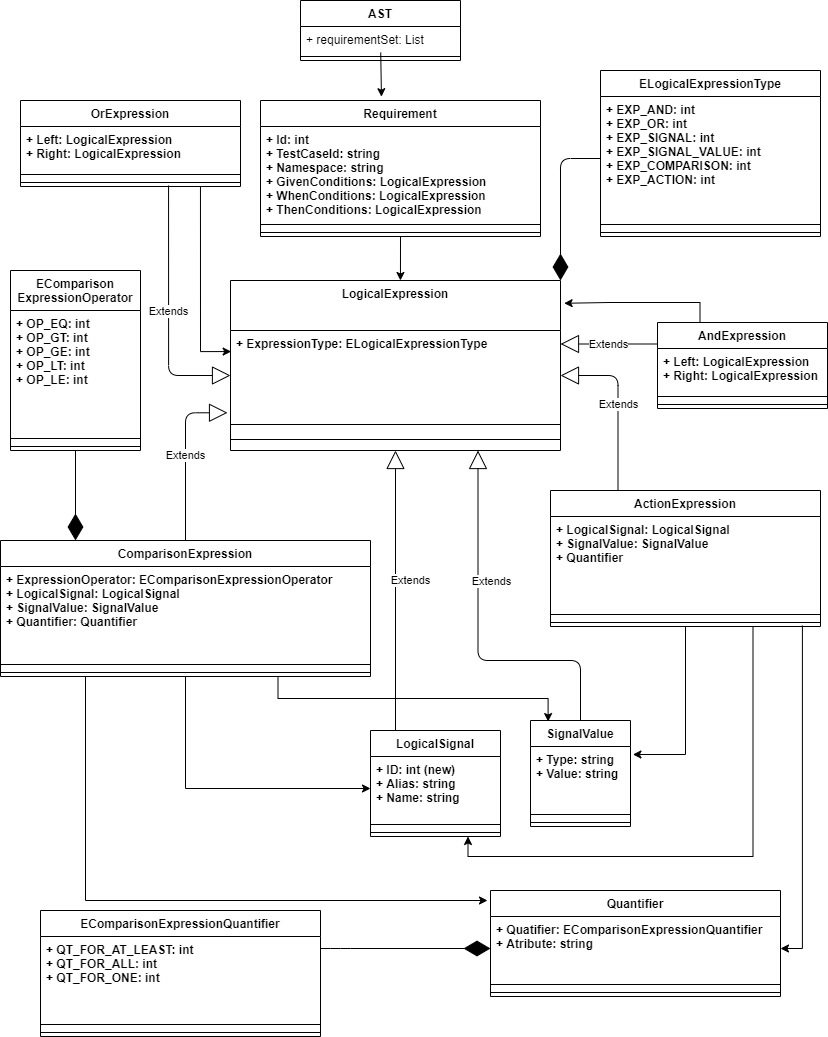
\includegraphics[width=\textwidth]{images/grammar_class_diagram.drawio.png}
    \caption{AST Class Diagram}
    \label{fig:ast_class_diagram}
\end{figure}

The defined grammar also supports the use of comments in the input file in the format of line comment or block-comment, "//" and "/**/" respectively.\\
The AST on Figure \ref{fig:ast_class_diagram} implements a list of requirements with as many as uncommented on the input file. The type of each expression is given by the ELogicalExpressionType enumerator. \textit{AndExpression} and \textit{OrExpression} are the defined boolean operators, however, Sesnando will report a warning message when an "OR" is used, as it usage is not advised according to Railway original requirement guidelines. A \textit{ComparisonExpression} is used for \textit{GIVEN} and \textit{WHEN} predicates and the \textit{ActionExpression} on \textit{THEN} predicates, as they define the output actions of a requirement, i.e., the expected results.


\subsection{Test case generation}
%----------------------- Command Line Inputs ----------------------------
\label{subsec:def_test_case_gen}

The process that generates a test specification is fully described on Section \ref{subsec:test_generation}. This section presents this process on the implementation level. For presentation purposes REQ466-1 is be given as an example.\\

\begin{Verbatim}[xleftmargin=12mm, numbers=left]
REQUIREMENT(REQ466-1, 2F02_Traction_Braking, CCUS)
{
	GIVEN <Train speed> is greater than 3
	    and <Brake Applied> is equal to true 
	    for at least one brake in the Unit;
	WHEN;
	// Juridical Recording Unit
	THEN <JRU Dragging Brake Detected> is set to true;
}
\end{Verbatim}

In order to register this event (a dragging brake has been detected on the train unit) to the Juridical Recording unit, it is needed to actually verify that the train is at Speed (greater than 3 kph) and there is at least one brake applied. This can be represented using a cause-effect-graph \cite{nursimulu_cause-effect_1995} on Figure \ref{fig:ceg_dbd}.

\begin{figure}[h]
    \centering
    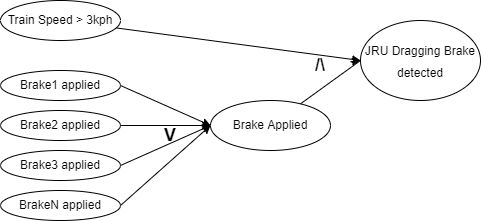
\includegraphics[width=\textwidth]{images/ceg_dbd.png}
    \caption{CEG of Dragging Brake detection}
    \label{fig:ceg_dbd}
\end{figure}


\textit{Sesnando} extracts all the Requirement signals by traversing the Parsed Object Tree (See Figure \ref{fig:req_parse_tree} and Figure \ref{fig:ast_class_diagram}) and for each, requests the corresponding Technical Signals from the Signal Manager using an API endpoint (api/signal/*Requirement Signal*) where *Requirement signal* is the actual Requirement Signal name from the input requirement.\\

As per MCDC, every input condition is a decision shall generate every possible outcome. As such, taking into consideration that one requirement signal might translate into multiple technical signals, when a clause states that at least one mapped technical signal should evaluate to true, the OR operator between these resulting technical signals is implicit (Equation \ref{eq:qt_or}). Otherwise, when all the technical signals are needed to evaluate to true for the clause outcome to be true, the AND operator amongst the technical signal is implicit (\ref{eq:qt_and}).


\begin{equation} \label{eq:qt_or}
    \text{Req. Signal on for-at-least-one (OR)} = \quad \forall tec.signal \in \{0 \lor 1 \lor 2 \dots \lor n-1\}
\end{equation}

\begin{equation} \label{eq:qt_and}
    \text{Req. Signal on for-all (AND)} = \quad \forall tec.signal \in \{0 \land 1 \land 2 \dots \land n-1\}
\end{equation}

Meaning that when a Requirement Signal maps to multiple technical signals, and in order to exercise every possible outcome, for the Equations above \textit{Sesnando} expands every requirement signals into multiple test steps in form of an Identity matrix NxN, where N is the number of technical signals, these scenarios are illustrated on Equations \ref{eq:m_qt_or} and \ref{eq:m_qt_and}, where a quantifier containing an implicit OR operator (e.g. for at least) is given by variable qtOR, whereas, a quantifier where an AND operator is implicit is defined as qtAnd. Considering that a Requirement signal maps to three (3) technical signals.


\begin{equation} \label{eq:m_qt_or}
qtOR (true) =
\begin{pmatrix}
1 & 0 & 0\\
0 & 1 & 0\\
0 & 0 & 1
\end{pmatrix}
\end{equation}

\begin{equation} \label{eq:m_qt_and}
qtAND (false) =
\begin{pmatrix}
0 & 1 & 1\\
1 & 0 & 1\\
1 & 1 & 0
\end{pmatrix}
\end{equation}

It is important to mention that when a requirement signal maps to multiple technical signals and the quantifier is omitted, the default behavior is the use of a "for all" quantifier, where all the mapping technical signals should be set or evaluate according to the values defined on the requirement (e.g. True).
As per MCDC, defining a different outcome for each clause presented on Equations \ref{eq:m_qt_or} and \ref{eq:m_qt_and} is given by Equations \ref{eq:m_qt_or_al}.

\begin{equation} \label{eq:m_qt_or_al}
qtOR (false) =
\begin{pmatrix}
0 & 0 & 0\\
\end{pmatrix}
\end{equation}

\begin{equation} \label{eq:m_qt_and_al}
qtAND (true) =
\begin{pmatrix}
1 & 1 & 1\\
\end{pmatrix}
\end{equation}

This means that a Predicate clause needs to consider the tests from Equations \ref{eq:m_qt_or}, \ref{eq:m_qt_and}, \ref{eq:m_qt_or_al} and \ref{eq:m_qt_and_al}. Thus, the requirement REQ466-1, results on the test Table \ref{tab:dbd_test_spec_m}.

\begin{table}[h]
\caption{Test Spec JRU Dragging Brake Detected}
    \footnotesize
    \centering
    
    \begin{tabular}{c c c c c c c}
        \hline
        % --- ROW Header --- %
        \textbf{\textit{Test step}} & 
        \textbf{\textit{TS}} & 
        \textbf{\textit{Bk1}} & 
        \textbf{\textit{Bk2}} & 
        \textbf{\textit{Bk3}} & 
        \textbf{\textit{Bk4}} & 
        \textbf{\textit{JRU DBkDet}}\\ \hline  \\
        
        % --- ROW 1 --- %
        \begin{tabular}[c]{@{}c@{}} \textbf{\textit{ 1 }} \end{tabular} & 
        4 & 
        0 &
        0 &
        0 &
        0 &
        0 \\
        \hline \\
        
        % --- ROW 2 --- %
        \begin{tabular}[c]{@{}c@{}} \textbf{\textit{ 2 }} \end{tabular} & 
        3 &
        1 &
        0 &
        0 &
        0 &
        0 \\
        \hline \\
       
        % --- ROW 3 --- %
        \begin{tabular}[c]{@{}c@{}} \textbf{\textit{ 3 }} \end{tabular} & 
        4 &
        1 &
        0 &
        0 &
        0 &
        1 \\
        \hline \\
        
        % --- ROW 4 --- %
        \begin{tabular}[c]{@{}c@{}} \textbf{\textit{ 4 }} \end{tabular} & 
        4 &
        0 &
        1 &
        0 &
        0 &
        1 \\
        \hline \\
        
        % --- ROW 5 --- %
        \begin{tabular}[c]{@{}c@{}} \textbf{\textit{ 5 }} \end{tabular} & 
        4 &
        0 &
        0 &
        1 &
        0 &
        1 \\
        \hline \\
        
        % --- ROW 6 --- %
        \begin{tabular}[c]{@{}c@{}} \textbf{\textit{ 6 }} \end{tabular} & 
        4 &
        0 &
        0 &
        0 &
        1 &
        1 \\
        \hline \\
        
    \end{tabular}
    \label{tab:dbd_test_spec_m}
\end{table}

Where \textbf{qtOR} is demonstrated to be present on tests 3 to 6. The evaluation of the outcome of the train speed is obtained by visiting the corresponding Requirement signal node within the Parsed object tree, and calling an eval() method that returns the limit values to test, determining the outcome of the clause containing train speed, where setting a value of 3 evaluates the clause to false and a value of 4 evaluates the clause to be true.


\subsection{Signal Manager Architecture}
%----------------------- Signal manager ----------------------------
\label{subsec:method_signal_manager}

As previously stated, it is intended that Signal Manager could be run as a detached service from the local compiler solution. This would allow that every tester, developer or involved user could contribute to the growth of information in it, such that every piece of testing information would be added only once, thus, the Test Generator accesses this remote repository in order to generate its tests, contributing to efficiently reduce the efforts needed, otherwise, every signal would need to be added as much as every existing localhost solutions.\\
The Signal manager acts as a Web Service and serves the Signal Manager through a REST API. There are several endpoints to consult, edit and create additional signals on the database. The purpose of these API Endpoints is not only to support Test Generator, but also the management of the signal data without the need of accessing the web user interface, e.g, automating the import of huge chunks of signal data. The Signal Manager contains fourteen database tables which supports the logic described throughout this report. An excerpt of this database can be observed on Fig. ~\ref{fig:db_signal_manager}.

\begin{figure}[H]
    \centering
    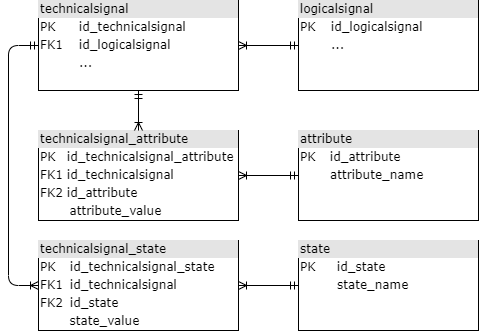
\includegraphics[scale=0.7]{images/signal_manager.png}
    \caption{Signal Manager DB Architecture (Excerpt)}
    \label{fig:db_signal_manager}
\end{figure}

A Logical Signal maps to one or more technical signals and a technical signal supports multiple attributes and states. A train Brake can be used as an example, as a possible attribute would be the location of this Brake within the train (Car=1,2..N) and its Axle (Axle=1..2), given that a train Car might contain two axles and a possible state would be whether this brakes are released or not (state="released", "not released") the latter usually maps to an integer value to represent the state, i.e, 1 or 0. This information is cross-checked on the Test Generator to process the correct technical signals according to the requirement information.


\subsection{Test Designer}
%----------------------- Signal manager ----------------------------
\label{subsec:method_test_designer}

The main benefits the test designer is the ability of the user to visualise the contents the test specification. By default, the test generator persists the test specification on a CSV file, so, without a Graphical User Interface, the user would have to rely on external tools in order to review it. In other words, the Test Designer loads the CSV contents into a grid-view where several operations might be executed, such as editing and saving this CSV file or generate test scripts.
